\documentclass[11pt, oneside]{article} 
\usepackage[margin=1in]{geometry}  
\geometry{letterpaper}
\usepackage{graphicx}		
\usepackage{amssymb}
\usepackage[parfill]{parskip}
\usepackage{amssymb}
\usepackage{amsmath}
\usepackage{listings}
\usepackage{color}
\usepackage{standalone}
\usepackage{gensymb}
\usepackage{tikz}
\usetikzlibrary{matrix,chains,positioning,decorations.pathreplacing,arrows}
\usepackage{wrapfig}

\graphicspath{ {images/} }

\def\layersep{2.5cm}

\sloppy
\definecolor{lightgray}{gray}{0.5}
\setlength{\parindent}{0pt}
\definecolor{dkgreen}{rgb}{0,0.6,0}
\definecolor{gray}{rgb}{0.5,0.5,0.5}
\definecolor{mauve}{rgb}{0.58,0,0.82}

\lstset{frame=tb,
  language=Matlab,
  aboveskip=3mm,
  belowskip=3mm,
  showstringspaces=false,
  columns=flexible,
  basicstyle={\small\ttfamily},
  numbers=none,
  numberstyle=\tiny\color{gray},
  keywordstyle=\color{blue},
  commentstyle=\color{dkgreen},
  stringstyle=\color{mauve},
  breaklines=true,
  breakatwhitespace=true,
  tabsize=3
}

\title{Neuro 120 Homework 1: Math and Hodgkin \& Huxley}
\author{William Schmitt and Will Drew}
\date{Due: Thursday 4 October 2018 at 5pm}

\begin{document}
\maketitle

\section{Question 1: Numerical Integration}

\subsection{Implement Euler Integration}
We implement Euler Integration as follows in Matlab:
\lstinputlisting{euler_solver.m}

\begin{figure}[ht!]
\centering
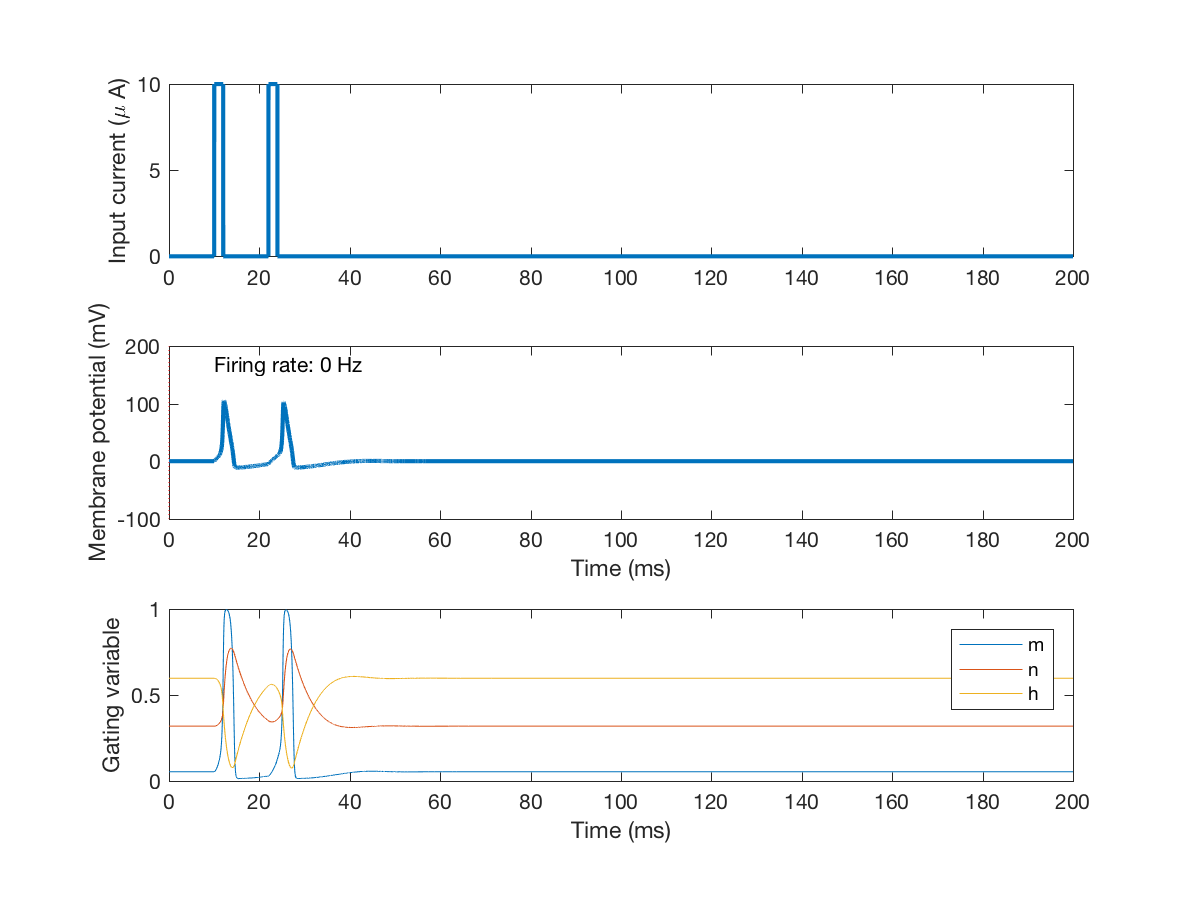
\includegraphics[width=1\textwidth]{simulate_hh_dt_1.eps}
\caption{Result of Euler Integration with $\Delta t = 0.01$.}
\label{fig:euler_integration_one}
\end{figure}

After changing line $29$ in \lstinline{simulate_hh.m} to \lstinline{use_euler=true}, we produce Figure \ref{fig:euler_integration_one}:

\subsection{Test Euler Integration Step Size}
We alter the setting of $\Delta t$ in \lstinline{simulate_hh.m} to $0.09$ and $0.07$ (e.g. change line 33 to \lstinline{dt = .09} or \lstinline{dt = .07}, respectively) and obtain Figures \ref{fig:euler_integration_nine} and \ref{fig:euler_integration_seven}, respectively. We see from these figures that having a step size of $0.09$ results in a failed simulation, which shows the membrane potential of the neuron going to negative infinity. This looks like it is the result of a gating variable ($m$) going to $-1$ in response to current stimulation.

Alternatively, when we set the step size to $0.07$, we get a simulation that looks from afar like it properly models the neural response, but upon close inspection, we can see that during the repolarization stage of the action potential, the model results in large oscillations. This indicates to us that we have too large a step size and need a smaller one in order to properly approximate the derivative of the gating variables.

\begin{figure}[ht!]
\centering
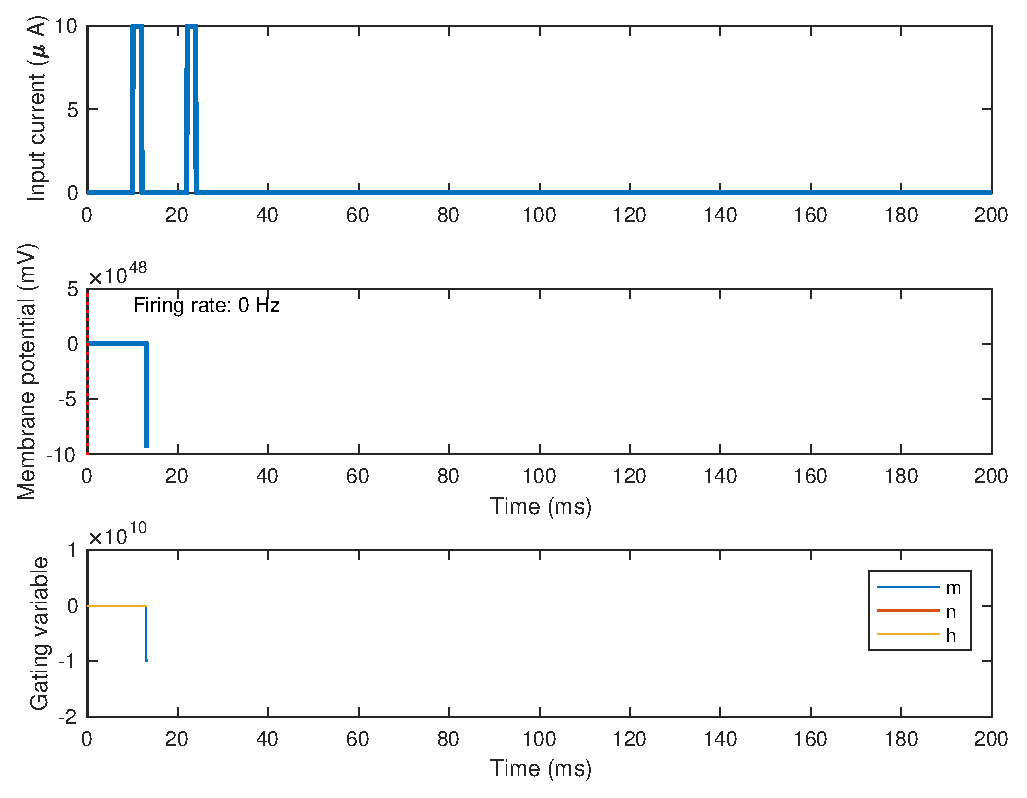
\includegraphics[width=1\textwidth]{simulate_hh_dt_9.eps}
\caption{Result of Euler Integration with $\Delta t = 0.09$.}
\label{fig:euler_integration_nine}
\end{figure}

\section{Question 2: Basic Spike Generation}
We zoom in (by using the figure tools) to the first action potential that is generated using our Euler integration model and display this in Figure \ref{fig:action_potential_close_up}. This figure illustrates how our simulated action potential slowly increases in membrane potential while there is an input current of $10\mu A$ until it hits the threshold for activation around a membrane potential of $20mV$. This activity is the result of the gating variable $m$ (which mimics the activation of a sodium channel) as we can see a similar rise in its value. After the rapid increase in the membrane potential, we see there is a rapid rise in the probability of finding a potassium channel activated (or open), which is shown by gating variable $n$. Somewhat delayed to this opening of potassium channels, the sodium channel inactivation probability increases (given by $1-h$). The combination of these two events begin to lower the membrane potential rapidly. Looking again at $m$, we see that most of the sodium channels rapidly become inactive, and now the only effect on the membrane potential is from the gating variables $n$ and $h$. These two gating variables slowly return to baseline, which results in a hyperpolarization of the membrane potential that slowly returns to baseline.

\section{Question 3: Firing Rate for Constant Inputs}

\subsection{The Relationship Between Firing Rate and Applied Input Current}



\subsection{Minimum Sustained Firing Rate}

\section{Question 4: Refractory Period}

\begin{figure}[ht!]
\centering
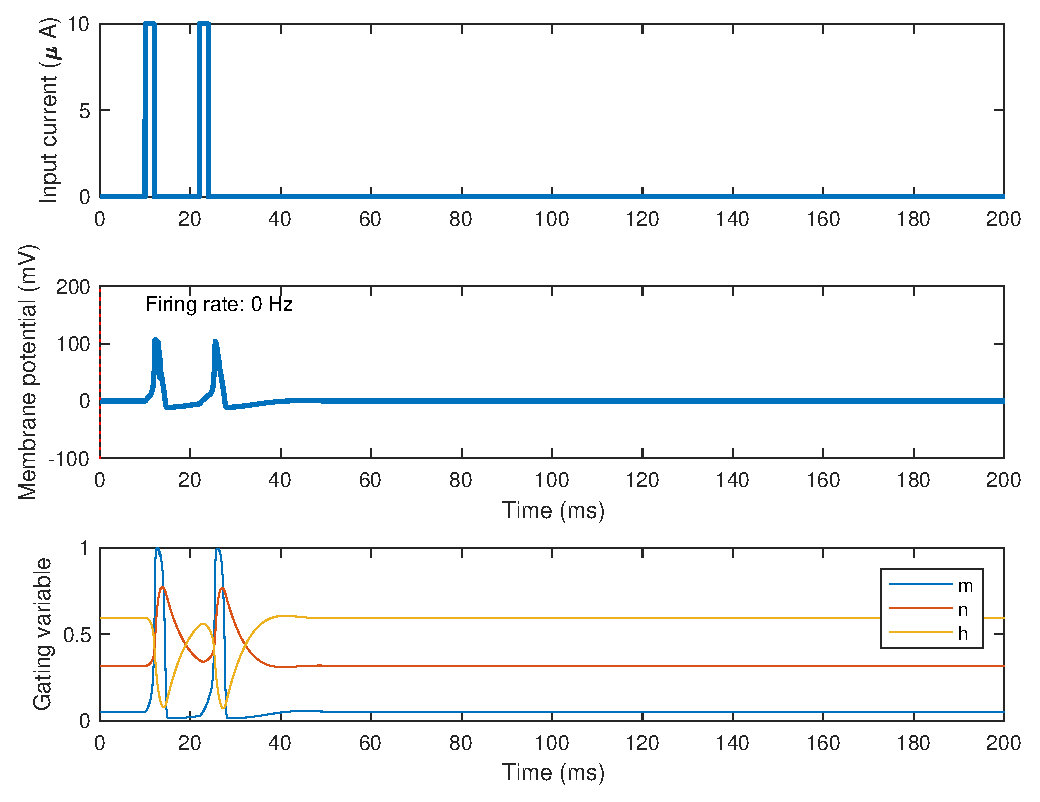
\includegraphics[width=1\textwidth]{simulate_hh_dt_7.eps}
\caption{Result of Euler Integration with $\Delta t = 0.07$.}
\label{fig:euler_integration_seven}
\end{figure}

\subsection{Spikes Fired for 12ms Pulse Separation}

\subsection{Spikes Fired for 3ms Pulse Separation}

\section{Question 5: History Dependence}

\begin{figure}[ht!]
\centering
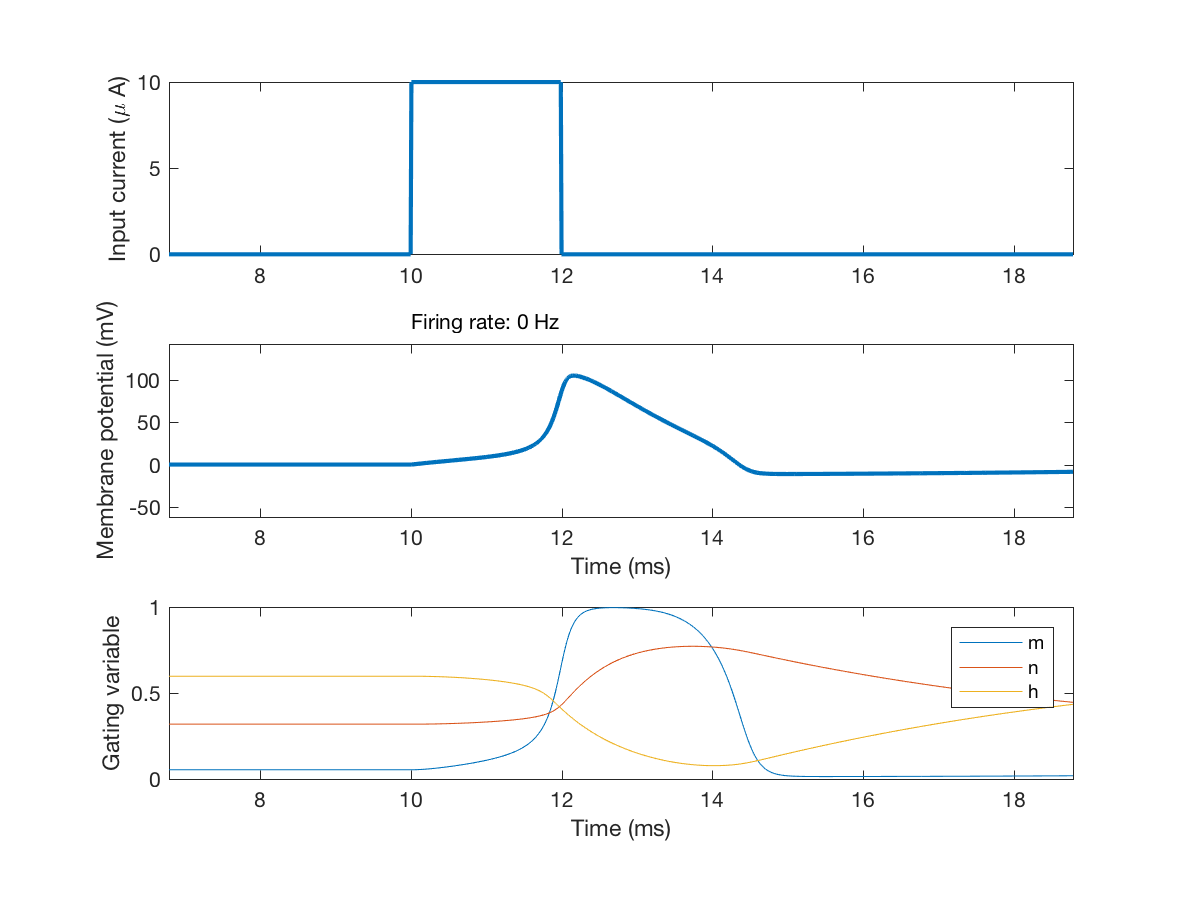
\includegraphics[width=1\textwidth]{simulate_hh_action_potential.eps}
\caption{A close-up look of a simulated action potential. Generated using the Euler integration model created in Question 1.}
\label{fig:action_potential_close_up}
\end{figure}

\subsection{Effects of Increasing Current on Firing Rate}

\subsection{Effects of Decreasing Current on Firing Rate}

\subsection{Firing Rate Curve for $10\mu A$ to $15\mu A$}

\subsection{Effects of Turning the Current Off on Firing Rate}

\section{Question 6: Oscillations}

\subsection{Manipulation of $\omega$}

\subsection{Firing Rate Dependence on $I_0$}

\subsection{Manipulation of $I_0$}

\section{Question 7: Extra Credit: Leaky Integration}



\end{document}